\chapter{气压与天气}\label{ch:g5:air-pressure-weather}

你生活在一片“空气海洋”的底部，这片海洋深达数百千米，
它的全部重量都压在你的肩上。
为什么它没有把你压垮？你为什么甚至感觉不到它？
这一切与明天的天气又有什么关系？空气这位看不见的老朋友，
还有一个重大的秘密等待揭开。

\section{空气有重量}

\begin{example}[称一称看不见的东西]\label{ex:g5:air-pressure-weather:weighing}
把一个充气很足的足球放在精密的天平上，使天平恰好平衡。
然后打开气门，多余的空气嘶嘶地跑出来——
还是同一个球、同一个气门，只是少了一些空气。
再放回天平称一称：瘪了的球\emph{更轻}。
两者的差值就是跑掉的空气的重量。
空气也是物质，物质有质量，地球会把质量往下拉；头顶的大气层因此是有重量的。
\end{example}

\begin{definition}[大气层与气压]\label{def:g5:air-pressure-weather:pressure}
\emph{大气层}\index{大气层}是包裹着整个地球的厚厚一层空气，
它的重量挤压着底部的空气（也就是我们生活的地方），
被挤压的空气会用力推向所接触的每一个表面。
这种推力称为\emph{气
压}\index{气压}。
\end{definition}

\begin{proposition}[来自各方的推力]\label{prop:g5:air-pressure-weather:allsides}
气压从\emph{各个}方向压迫每一个表面，
向下压桌面，向侧面压墙壁，甚至\emph{向上}压天花板和手掌。
气压的威力很大：在一个手掌大小的面积上，
空气的推力约等于一只又大又满的行李箱的重量。
我们却从不觉得，因为各方向的推力相互平衡：
人体内部和每个表面另一侧的空气，同样用力地向外推。
\end{proposition}

\begin{method}[托住水的硬纸片]\label{met:g5:air-pressure-weather:card}
空气向上的推力，被我们当场“逮个正着”（请在水槽上方做这个实验）：
\begin{enumerate}
  \item 在杯子里装满水，直至水面与杯口齐平；
  \item 在杯口上平放一张硬而光滑的卡片，
        卡片四周都要紧贴水面；
  \item 用手按住卡片，把杯子整个倒过来，
        然后轻轻松开卡片。
\end{enumerate}
卡片没有掉下来——它托住了整杯水。水的重量向下压着卡片，
但大气层压着它的力更大。
大气层的推力是\emph{向上}的。你刚刚看到了“行李箱”式的推力，
从下方把卡片托住了。
\end{method}

\begin{omfigure}
\begin{tikzpicture}[scale=0.85]
  \draw[thick] (4.4,1.2) -- (4.4,3.6) (6.6,1.2) -- (6.6,3.6);
  \draw[thick] (4.4,3.6) -- (6.6,3.6);
  \fill[omDef, opacity=0.25] (4.4,1.25) rectangle (6.6,3.55);
  \draw[very thick, omMeth] (4.25,1.2) -- (6.75,1.2);
  \node[right, font=\small, omMeth] at (6.9,1.2) {卡片};
  \draw[-Stealth, thick, omDef] (5.0,2.9) -- (5.0,2.2);
  \draw[-Stealth, thick, omDef] (6.0,2.9) -- (6.0,2.2);
  \node[above, font=\small, omDef] at (5.5,3.65)
    {水向下压};
  \foreach \x in {4.7,5.5,6.3} {
    \draw[-Stealth, very thick, omThm] (\x,0.15) -- (\x,0.95);
  }
  \node[below, font=\small, omThm] at (5.5,-0.05)
    {大气层向上推——而且更用力};
\end{tikzpicture}

{\small 倒扣的杯子：空气向上作用于卡片的推力
胜过了水的重量。看不见的“空气海洋”力量可真不小。}
\end{omfigure}

\section{大气层推动的“机器”}

\begin{example}[吸管]\label{ex:g5:air-pressure-weather:straw}
你以为是自己把果汁“吸”上了吸管。其实，你根本没法拉动液体——
不信就试试用手指去拉水！你真正做的是
把吸管里的\emph{空气}吸出来。吸管里的空气被吸走后，
大气层压在杯中果汁的表面上，
便把果汁沿着空吸管推送到你嘴边。每一口都是
大气层在“托举”；你只是替它清了路。
\end{example}

\begin{example}[吸盘与被压扁的瓶子]\label{ex:g5:air-pressure-weather:suction}
浴室挂钩的橡胶吸盘被紧紧压在瓷砖上，
把下面的空气挤了出去：这时大气层
把吸盘压向墙面，而吸盘背后没有空气顶回来——
吸盘就这样被天空“按”在墙上。再把瓶盖拧紧在一个空的塑料瓶上，
带到高山上，然后开车下到山谷：
瓶子就像被无形的手捏扁了一样。瓶外的空气
压力比封在瓶里的高山稀薄空气大得多——
大气层占了上风，瓶子就瘪了。
\end{example}

\begin{example}[越高越稀薄]\label{ex:g5:air-pressure-weather:height}
向上攀登，你就把一部分“空气海洋”留在了下面：
上方的空气少了，推力也就弱了。乘坐快速缆车时，
外部气压在变化，你的耳朵会突然“嘭”的一下；登山者则要大口喘息，吸入越来越稀薄的空气。
去年那个山顶上“煮茶不开”的谜团也就解开了：大气层压在水面上的力变小，
水就更容易沸腾——
在高山之巅，水的沸点远低于\qty{100}{\celsius}，
水温太低，泡不出像样的茶。
\end{example}

\begin{omfigure}
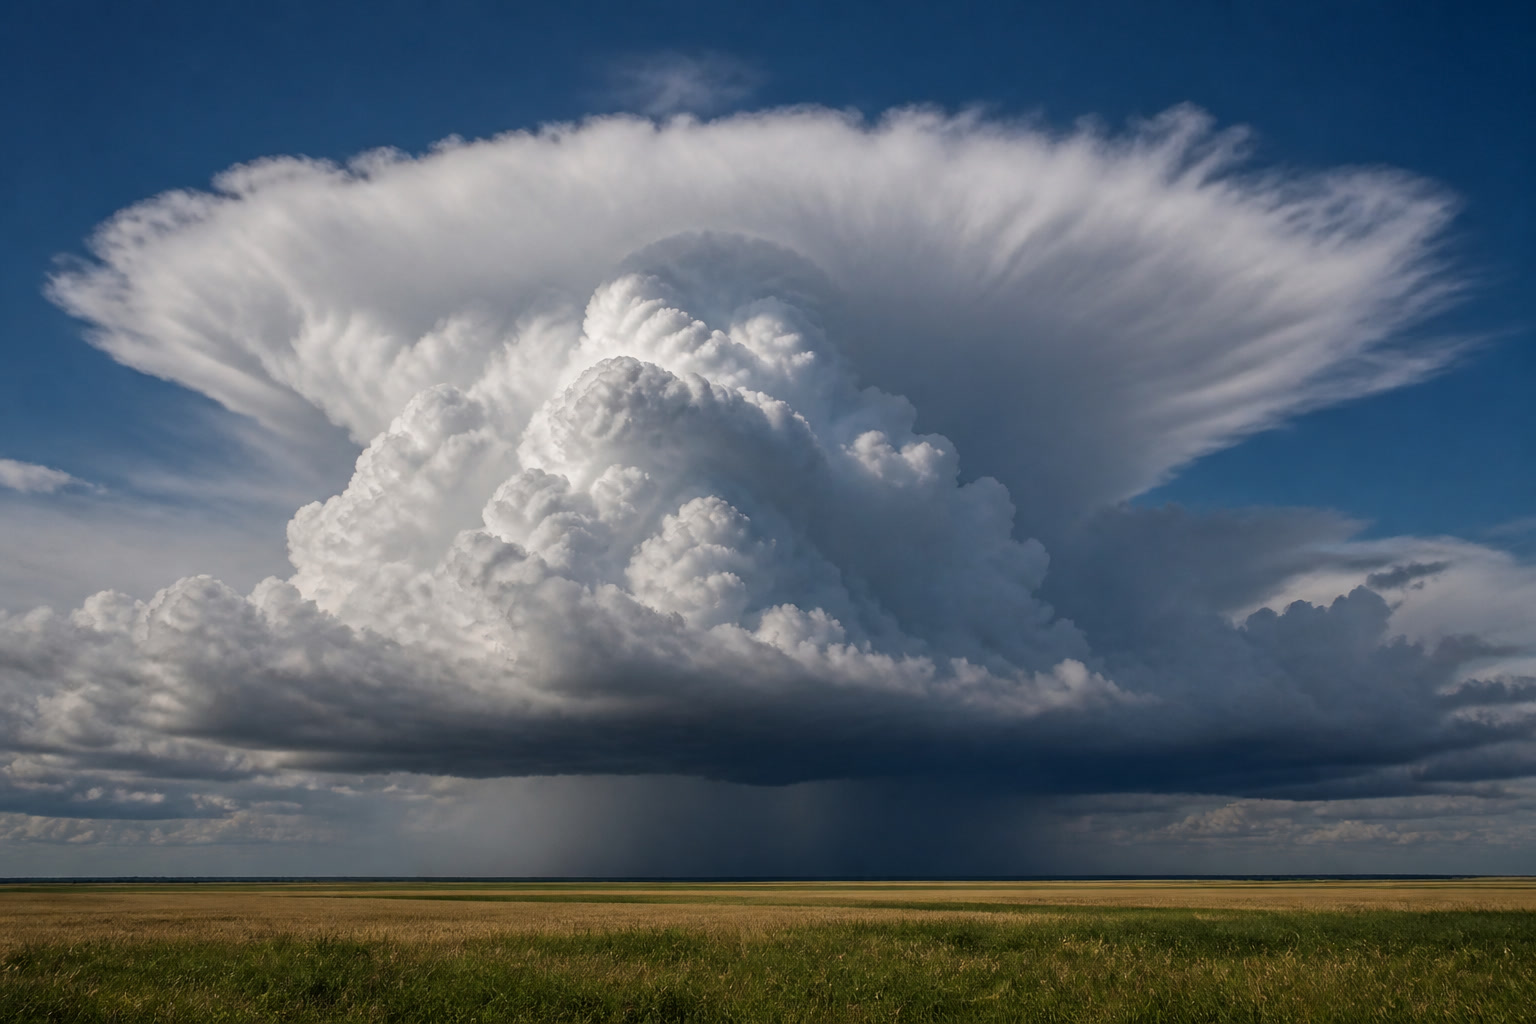
\includegraphics[width=0.58\linewidth]{images/book1/ai/g5-weather-storm.jpg}

{\small 雷雨云高耸在田野上方：天气就是流动的大气层。}
\end{omfigure}

\section{气压计与天气}

\begin{definition}[气压计]\label{def:g5:air-pressure-weather:barometer}
\emph{气压计}\index{气压计}是用来测量
气压的仪器 --- 它是我们“诚实法官”家族的又一员，
与温度计、天平并列。
上方的大气层压得更重时，指针上升；
压力减小时，指针下降。
\end{definition}

\begin{proposition}[气压预示明天的天气]\label{prop:g5:air-pressure-weather:weather}
大气层的气压总在变化：下沉的重空气带来
平静晴朗的天气；上升的轻空气则带来云和雨。因此，
气压计是一位朴实诚实的“预言家”：
\emph{稳定或上升}的气压预示天气晴好；
\emph{下降}的气压预示云层将至；\emph{快速下降}
则意味着暴风雨可能正在途中。
\end{proposition}

\begin{omfigure}
\begin{tikzpicture}[scale=0.85]
  \draw[thick] (2.2,1.7) circle (1.5);
  \foreach \a/\t in {150/{}, 120/{}, 90/{}, 60/{}, 30/{}} {
    \draw (2.2,1.7) ++(\a:1.3) -- ++(\a:0.18);
  }
  \node[font=\footnotesize] at (1.1,2.6) {雨};
  \node[font=\footnotesize] at (2.2,3.0) {变化};
  \node[font=\footnotesize] at (3.4,2.6) {晴};
  \draw[-Stealth, very thick, omThm] (2.2,1.7) -- ++(55:1.1);
  \fill (2.2,1.7) circle (2pt);
  \node[below, font=\small] at (2.2,-0.05)
    {家用气压计：指针偏向晴};
  \node[right, font=\small, align=left] at (5.4,2.5)
    {指针上升：前方晴朗};
  \node[right, font=\small, align=left] at (5.4,1.7)
    {指针下降：云层聚集};
  \node[right, font=\small, align=left] at (5.4,0.9)
    {快速下降：做好防风准备 --- 暴风雨};
\end{tikzpicture}

{\small 读气压计：与其看指针停在哪里，
不如看它往哪边动 --- 大气层在宣告它的计划。}
\end{omfigure}

\begin{remark}[天气图上的 H 与 L]\label{rem:g5:air-pressure-weather:map}
今晚的天气预报会显示标有 H 与 L 的大漩涡：
高压区和低压区像慢悠悠的鲸鱼，
在地图上缓缓漂移。空气总是从沉重的 H 区域流向
轻盈的 L 区域 --- 这种流动\emph{就是风}。本章一次讲清三位老朋友：
气压计的预报、风的起源，
以及你的耳朵为何能察觉
天气即将转变。
\end{remark}

\section{练习}

\begin{exercise}[$\star$]\label{exo:g5:air-pressure-weather:1}
足球实验如何说明空气有重力？
究竟比较了什么？
\end{exercise}

\begin{exercise}[$\star$]\label{exo:g5:air-pressure-weather:2}
什么是气压？它从哪里来？
它沿哪些方向施压？
\end{exercise}

\begin{exercise}[$\star$]\label{exo:g5:air-pressure-weather:3}
大气在你的手掌上施加的压力，大约相当于一只装满的
行李箱的重量 --- 你却毫无感觉。为什么？
\end{exercise}

\begin{exercise}[$\star$]\label{exo:g5:air-pressure-weather:4}
在卡片魔术中，两股力争夺这张卡片。
说出它们各是什么，并说明哪一个获胜。
\end{exercise}

\begin{exercise}[$\star$]\label{exo:g5:air-pressure-weather:5}
“我把果汁拉上吸管。”请改正这句话：
你真正除去了什么？是谁在把果汁抬起？
\end{exercise}

\begin{exercise}[$\star$]\label{exo:g5:air-pressure-weather:6}
吸盘为什么能吸住瓷砖？被挤出去的是什么，
又是什么使吸盘固定在上面？
\end{exercise}

\begin{exercise}[$\star$]\label{exo:g5:air-pressure-weather:7}
爬山时，气压会怎样变化？为什么？
请举出游客能够察觉到的两个迹象。
\end{exercise}

\begin{exercise}[$\star$]\label{exo:g5:air-pressure-weather:8}
气压计测量的是什么？你的气压计自早餐后
一直快速下降 --- 野餐计划应当预料到什么？
\end{exercise}

\begin{exercise}[$\star\star$]\label{exo:g5:air-pressure-weather:9}
密封的瓶子在从山上开车下来的途中瘪了。
请用瓶内、瓶外的压力解释瓶子变瘪的原因 --- 并
预测：若把一只密封的瓶子放在山谷中，再
带\emph{上山}，会发生什么？
\end{exercise}

\begin{exercise}[$\star\star$]\label{exo:g5:air-pressure-weather:10}
根据天气图上 H 与 L 的漩涡，风从哪里来？
请把它与本书最古老的定义联系起来：风是
流动的空气 --- 是什么推动了它？
\end{exercise}

\begin{exercise}[$\star\star$]\label{exo:g5:air-pressure-weather:11}
登山者抱怨说，在高峰上，茶永远泡不浓，
煮再久，意大利面也还是硬的。综合两年所学，给出完整解释：
稀薄的大气层对沸点有何影响？
为什么延长煮沸时间也无济于事？
（两条命题，其中一条来自去年，可解决这一问题。）
\end{exercise}
